\documentclass[12pt,a4paper]{article}
\usepackage[utf8]{inputenc}
\usepackage{amsmath}
\usepackage{amsfonts}
\usepackage{amssymb}
\usepackage[brazil]{babel}
\usepackage{indentfirst}
\usepackage{url}
\usepackage{listings}
\RequirePackage{graphicx}
\title{Alternativas de editores WYSIWYG}
\author{Daniel Moreira \and Gilvan Junior \and Jeferson Rosini \and Jônatas Rezende \and Jonathan \and Lara Caroline \and Lucas Pereira \and Luciano de Carvalho \and Maciele Xavier \and Macilon Arruda}
\usepackage[left=3cm,right=3cm,top=2cm,bottom=2cm]{geometry}
\usepackage{color}
    \definecolor{editorGray}{rgb}{0.95, 0.95, 0.95}
    \definecolor{editorOcher}{rgb}{1, 0.5, 0} % #FF7F00 -> rgb(239, 169, 0)
    \definecolor{editorGreen}{rgb}{0, 0.5, 0} % #007C00 -> rgb(0, 124, 0)
    \usepackage{upquote}
    \usepackage{listings}
    \lstdefinelanguage{JavaScript}{
      morekeywords={break, case, catch, continue, debugger, default, delete,         do, else, false, finally, for, function, if, in, instanceof, new, null, return, switch, this, throw, true, try, typeof, var, void, while, with},
      morecomment=[s]{/*}{*/},
      morecomment=[l]//,
      morestring=[b]",
      morestring=[b]'
    }
    \lstdefinelanguage{CSS}{
      keywords={accelerator,azimuth,background,background-attachment,
            background-color,background-image,background-position,
            background-position-x,background-position-y,background-repeat,
            behavior,border,border-bottom,border-bottom-color,
            border-bottom-style,border-bottom-width,border-collapse,
            border-color,border-left,border-left-color,border-left-style,
            border-left-width,border-right,border-right-color,
            border-right-style,border-right-width,border-spacing,
            border-style,border-top,border-top-color,border-top-style,
            border-top-width,border-width,bottom,caption-side,clear,
            clip,color,content,counter-increment,counter-reset,cue,
            cue-after,cue-before,cursor,direction,display,elevation,
            empty-cells,filter,float,font,font-family,font-size,
            font-size-adjust,font-stretch,font-style,font-variant,
            font-weight,height,ime-mode,include-source,
            layer-background-color,layer-background-image,layout-flow,
            layout-grid,layout-grid-char,layout-grid-char-spacing,
            layout-grid-line,layout-grid-mode,layout-grid-type,left,
            letter-spacing,line-break,line-height,list-style,
            list-style-image,list-style-position,list-style-type,margin,
            margin-bottom,margin-left,margin-right,margin-top,
            marker-offset,marks,max-height,max-width,min-height,
            min-width,-moz-binding,-moz-border-radius,
            -moz-border-radius-topleft,-moz-border-radius-topright,
            -moz-border-radius-bottomright,-moz-border-radius-bottomleft,
            -moz-border-top-colors,-moz-border-right-colors,
            -moz-border-bottom-colors,-moz-border-left-colors,-moz-opacity,
            -moz-outline,-moz-outline-color,-moz-outline-style,
            -moz-outline-width,-moz-user-focus,-moz-user-input,
            -moz-user-modify,-moz-user-select,orphans,outline,
            outline-color,outline-style,outline-width,overflow,
            overflow-X,overflow-Y,padding,padding-bottom,padding-left,
            padding-right,padding-top,page,page-break-after,
            page-break-before,page-break-inside,pause,pause-after,
            pause-before,pitch,pitch-range,play-during,position,quotes,
            -replace,richness,right,ruby-align,ruby-overhang,
            ruby-position,-set-link-source,size,speak,speak-header,
            speak-numeral,speak-punctuation,speech-rate,stress,
            scrollbar-arrow-color,scrollbar-base-color,
            scrollbar-dark-shadow-color,scrollbar-face-color,
            scrollbar-highlight-color,scrollbar-shadow-color,
            scrollbar-3d-light-color,scrollbar-track-color,table-layout,
            text-align,text-align-last,text-decoration,text-indent,
            text-justify,text-overflow,text-shadow,text-transform,
            text-autospace,text-kashida-space,text-underline-position,top,
            unicode-bidi,-use-link-source,vertical-align,visibility,
            voice-family,volume,white-space,widows,width,word-break,
            word-spacing,word-wrap,writing-mode,z-index,zoom},  
      sensitive=true,
      morecomment=[l]{//},
      morecomment=[s]{/*}{*/},
      morestring=[b]',
      morestring=[b]",
      alsoletter={:},
      alsodigit={-}
    }
    \lstdefinelanguage{HTML5}{
            language=html,
            sensitive=true, 
            alsoletter={<>=-},
            otherkeywords={
            % HTML tags
            <, </, >,
            </a, <a, </a>,
            </abbr, <abbr, </abbr>,
            </address, <address, </address>,
            </area, <area, </area>,
            </area, <area, </area>,
            </article, <article, </article>,
            </aside, <aside, </aside>,
            </audio, <audio, </audio>,
            </audio, <audio, </audio>,
            </b, <b, </b>,
            </base, <base, </base>,
            </bdi, <bdi, </bdi>,
            </bdo, <bdo, </bdo>,
            </blockquote, <blockquote, </blockquote>,
            </body, <body, </body>,
            </br, <br, </br>,
            </button, <button, </button>,
            </canvas, <canvas, </canvas>,
            </caption, <caption, </caption>,
            </cite, <cite, </cite>,
            </code, <code, </code>,
            </col, <col, </col>,
            </colgroup, <colgroup, </colgroup>,
            </data, <data, </data>,
            </datalist, <datalist, </datalist>,
            </dd, <dd, </dd>,
            </del, <del, </del>,
            </details, <details, </details>,
            </dfn, <dfn, </dfn>,
            </div, <div, </div>,
            </dl, <dl, </dl>,
            </dt, <dt, </dt>,
            </em, <em, </em>,
            </embed, <embed, </embed>,
            </fieldset, <fieldset, </fieldset>,
            </figcaption, <figcaption, </figcaption>,
            </figure, <figure, </figure>,
            </footer, <footer, </footer>,
            </form, <form, </form>,
            </h1, <h1, </h1>,
            </h2, <h2, </h2>,
            </h3, <h3, </h3>,
            </h4, <h4, </h4>,
            </h5, <h5, </h5>,
            </h6, <h6, </h6>,
            </head, <head, </head>,
            </header, <header, </header>,
            </hr, <hr, </hr>,
            </html, <html, </html>,
            </i, <i, </i>,
            </iframe, <iframe, </iframe>,
            </img, <img, </img>,
            </input, <input, </input>,
            </ins, <ins, </ins>,
            </kbd, <kbd, </kbd>,
            </keygen, <keygen, </keygen>,
            </label, <label, </label>,
            </legend, <legend, </legend>,
            </li, <li, </li>,
            </link, <link, </link>,
            </main, <main, </main>,
            </map, <map, </map>,
            </mark, <mark, </mark>,
            </math, <math, </math>,
            </menu, <menu, </menu>,
            </menuitem, <menuitem, </menuitem>,
            </meta, <meta, </meta>,
            </meter, <meter, </meter>,
            </nav, <nav, </nav>,
            </noscript, <noscript, </noscript>,
            </object, <object, </object>,
            </ol, <ol, </ol>,
            </optgroup, <optgroup, </optgroup>,
            </option, <option, </option>,
            </output, <output, </output>,
            </p, <p, </p>,
            </param, <param, </param>,
            </pre, <pre, </pre>,
            </progress, <progress, </progress>,
            </q, <q, </q>,
            </rp, <rp, </rp>,
            </rt, <rt, </rt>,
            </ruby, <ruby, </ruby>,
            </s, <s, </s>,
            </samp, <samp, </samp>,
            </script, <script, </script>,
            </section, <section, </section>,
            </select, <select, </select>,
            </small, <small, </small>,
            </source, <source, </source>,
            </span, <span, </span>,
            </strong, <strong, </strong>,
            </style, <style, </style>,
            </summary, <summary, </summary>,
            </sup, <sup, </sup>,
            </svg, <svg, </svg>,
            </table, <table, </table>,
            </tbody, <tbody, </tbody>,
            </td, <td, </td>,
            </template, <template, </template>,
            </textarea, <textarea, </textarea>,
            </tfoot, <tfoot, </tfoot>,
            </th, <th, </th>,
            </thead, <thead, </thead>,
            </time, <time, </time>,
            </title, <title, </title>,
            </tr, <tr, </tr>,
            </track, <track, </track>,
            </u, <u, </u>,
            </ul, <ul, </ul>,
            </var, <var, </var>,
            </video, <video, </video>,
            </wbr, <wbr, </wbr>,
            />, <!
            },  
            ndkeywords={
            % General
            =,
            % HTML attributes
            accept=, accept-charset=, accesskey=, action=, align=, alt=, async=, autocomplete=, autofocus=, autoplay=, autosave=, bgcolor=, border=, buffered=, challenge=, charset=, checked=, cite=, class=, code=, codebase=, color=, cols=, colspan=, content=, contenteditable=, contextmenu=, controls=, coords=, data=, datetime=, default=, defer=, dir=, dirname=, disabled=, download=, draggable=, dropzone=, enctype=, for=, form=, formaction=, headers=, height=, hidden=, high=, href=, hreflang=, http-equiv=, icon=, id=, ismap=, itemprop=, keytype=, kind=, label=, lang=, language=, list=, loop=, low=, manifest=, max=, maxlength=, media=, method=, min=, multiple=, name=, novalidate=, open=, optimum=, pattern=, ping=, placeholder=, poster=, preload=, pubdate=, radiogroup=, readonly=, rel=, required=, reversed=, rows=, rowspan=, sandbox=, scope=, scoped=, seamless=, selected=, shape=, size=, sizes=, span=, spellcheck=, src=, srcdoc=, srclang=, start=, step=, style=, summary=, tabindex=, target=, title=, type=, usemap=, value=, width=, wrap=,
            % CSS properties
            accelerator:,azimuth:,background:,background-attachment:,
            background-color:,background-image:,background-position:,
            background-position-x:,background-position-y:,background-repeat:,
            behavior:,border:,border-bottom:,border-bottom-color:,
            border-bottom-style:,border-bottom-width:,border-collapse:,
            border-color:,border-left:,border-left-color:,border-left-style:,
            border-left-width:,border-right:,border-right-color:,
            border-right-style:,border-right-width:,border-spacing:,
            border-style:,border-top:,border-top-color:,border-top-style:,
            border-top-width:,border-width:,bottom:,caption-side:,clear:,
            clip:,color:,content:,counter-increment:,counter-reset:,cue:,
            cue-after:,cue-before:,cursor:,direction:,display:,elevation:,
            empty-cells:,filter:,float:,font:,font-family:,font-size:,
            font-size-adjust:,font-stretch:,font-style:,font-variant:,
            font-weight:,height:,ime-mode:,include-source:,
            layer-background-color:,layer-background-image:,layout-flow:,
            layout-grid:,layout-grid-char:,layout-grid-char-spacing:,
            layout-grid-line:,layout-grid-mode:,layout-grid-type:,left:,
            letter-spacing:,line-break:,line-height:,list-style:,
            list-style-image:,list-style-position:,list-style-type:,margin:,
            margin-bottom:,margin-left:,margin-right:,margin-top:,
            marker-offset:,marks:,max-height:,max-width:,min-height:,
            min-width:,transition-duration:,transition-property:,
            transition-timing-function:,transform:,
            -moz-transform:,-moz-binding:,-moz-border-radius:,
            -moz-border-radius-topleft:,-moz-border-radius-topright:,
            -moz-border-radius-bottomright:,-moz-border-radius-bottomleft:,
            -moz-border-top-colors:,-moz-border-right-colors:,
            -moz-border-bottom-colors:,-moz-border-left-colors:,-moz-opacity:,
            -moz-outline:,-moz-outline-color:,-moz-outline-style:,
            -moz-outline-width:,-moz-user-focus:,-moz-user-input:,
            -moz-user-modify:,-moz-user-select:,orphans:,outline:,
            outline-color:,outline-style:,outline-width:,overflow:,
            overflow-X:,overflow-Y:,padding:,padding-bottom:,padding-left:,
            padding-right:,padding-top:,page:,page-break-after:,
            page-break-before:,page-break-inside:,pause:,pause-after:,
            pause-before:,pitch:,pitch-range:,play-during:,position:,quotes:,
            -replace:,richness:,right:,ruby-align:,ruby-overhang:,
            ruby-position:,-set-link-source:,size:,speak:,speak-header:,
            speak-numeral:,speak-punctuation:,speech-rate:,stress:,
            scrollbar-arrow-color:,scrollbar-base-color:,
            scrollbar-dark-shadow-color:,scrollbar-face-color:,
            scrollbar-highlight-color:,scrollbar-shadow-color:,
            scrollbar-3d-light-color:,scrollbar-track-color:,table-layout:,
            text-align:,text-align-last:,text-decoration:,text-indent:,
            text-justify:,text-overflow:,text-shadow:,text-transform:,
            text-autospace:,text-kashida-space:,text-underline-position:,top:,
            unicode-bidi:,-use-link-source:,vertical-align:,visibility:,
            voice-family:,volume:,white-space:,widows:,width:,word-break:,
            word-spacing:,word-wrap:,writing-mode:,z-index:,zoom:
            },  
            morecomment=[s]{<!--}{-->},
            tag=[s]
    }

    \lstset{%
        % Basic design
        backgroundcolor=\color{editorGray},
        basicstyle={\small\ttfamily},   
        frame=l,
        % Line numbers
        xleftmargin={0.75cm},
        numbers=left,
        stepnumber=1,
        firstnumber=1,
        numberfirstline=true,
        % Code design   
        keywordstyle=\color{blue}\bfseries,
        commentstyle=\color{darkgray}\ttfamily,
        ndkeywordstyle=\color{editorGreen}\bfseries,
        stringstyle=\color{editorOcher},
        % Code
        language=HTML5,
        alsodigit={.:;},
        tabsize=2,
        showtabs=false,
        showspaces=false,
        showstringspaces=false,
        extendedchars=true,
        breaklines=true,        
    }

\begin{document}
\begin{titlepage}


\begin{center}
\begin{figure}[htb]
		
		\label{figura:LogoIF}
	
		\centering
		
\includegraphics[width=6cm]{logo.png} 
\end{figure}


Instituto Federal Goiano - Campus Ceres\\
Bacharelado em Sistemas de Informação\\
Prof. Me. Ronneesley Moura Teles\\\vspace{0.2cm}
Daniel Moreira Cardoso \\
Jeferson Rossini Ferreira Lourenço\\
Jônatas de Souza Rezende\\
Jonathan Silvestre de Sousa\\
José Gilvan Jacinto Junior\\
Lara Caroline Damaceno Faria\\
Lucas Pereira de Azevedo\\
Luciano de Carvalho Borba\\
Maciele Xavier Rodrigues \\
Macilon Arruda Peixoto\\



\vspace{5.0cm}

\textit{\textbf{\Large{Alternativas de editores WYSIWYG}}}\\\vspace{0.5cm}
\vspace{9.5cm}

Setembro\\
2017\\
\end{center}
\end{titlepage}



\tableofcontents

\newpage
\begin{center}
\textbf{\Large{Alternativas de editores WYSIWYG}}\\\vspace{0.5cm}
\end{center}

\section{Introdução}

WYSIWYG (what You See Is What You Get – O que você vê é o que você obtém) são ferramentas de edição e desenvolvimento que funcionam em tempo real, em que, permitem visualizar o mesmo que será impresso. O exemplo mais simples e claro são os editores de texto, word e writer.

Atualmente estes recursos são utilizados em larga escala, já que possibilitam o manejo de textos e outras funcionalidade como: Inserção de links, vídeos, imagens, tabelas, iframes e uma infinidade de personalizações.

Utilizando este recurso, é possível que um usuário comum possa personalizar de maneira mais amigável seus posts sem ter conhecimento algum sobre qualquer linguagem de programação. 

Nossa Rede Social possui áreas específicas para publicação de conteúdo, seja ele publicação simples ou “aportes” que são na maioria das vezes conteúdos que utilizam tabelas, marcações e outros tipos de cabeçalho para determinadas sessões dentro do texto.

 Logo se faz necessária a utilização deste recurso dentro da nossa rede social, por esse motivo separamos 4 WYSIWYG mais utilizados e gratuitos para nosso projeto:


\section{TinyMCE}
O TinyMCE  é um editor bem simples porém eficiente, foi projetado para se integrar facilmente a sistemas de gerenciamento de conteúdo, versão estável 4.5.7, lançada em 25 de abril de 2017 como open-source sob licença LGPL, ele é compatível com os navegadores google chrome, mozilla, firefox, safari, Microsoft Edge e internet explorer, em vários sistemas operacionais.

O suporte comunitário peer-to-peer para o TinyMCE pode ser encontrado nos fóruns, ele também possui uma grande quantidade de  plugins, e extremamente fácil de ser configurado, apesar de ser leve é bem completo. 

\subsection{Vantagens}
\begin{enumerate}
\item Copiar melhorado
\begin{itemize}
\item Tecnologia incomparável que limpa suas senhas Conteúdo do Word e combina estilos de acordo com suas preferências (também funciona com imagens).
\end{itemize}
\item Verificação ortográfica
\begin{itemize}
\item Permita que seus usuários vejam os erros de digitação à medida que eles digitam. Os erros podem ser corrigidos em tempo real escolhendo a palavra mais apropriada.
\end{itemize}
\item Gerenciamento de arquivos
\begin{itemize}
\item Com base no nosso produto MoxieManager, você pode carregar e gerenciar arquivos no Microsoft Azure, Google Drive, Amazon S3, DropBox e muito mais.
\end{itemize}
\end{enumerate}

\subsection{Como utilizar?}
\begin{enumerate}
\item Faça a inclusão do plugin no header do seu documento html.
\lstinputlisting{recursos/TinyMCE/Step1.html}

\item Defina o selector para que o tinymce consiga transformar a textarea em um recurso editor WYSIWYG.
\lstinputlisting{recursos/TinyMCE/Step2.html}
\end{enumerate}

\subsection{Resultado}

\begin{figure}[h]
\centering
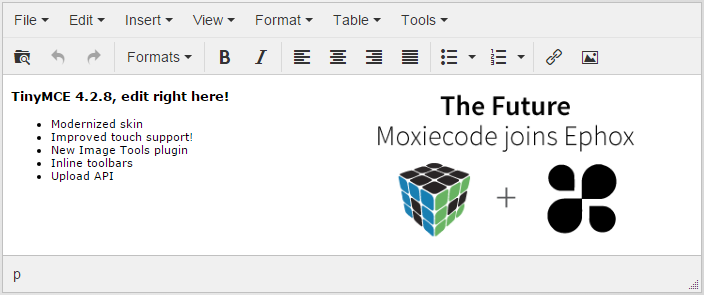
\includegraphics[width=13cm]{recursos/TinyMCE/TinyMCE.png}
\label{1}
\caption{TinyMCE. Fonte:https://goo.gl/ZkHeX1; Acesso em 22/09/2017}
\end{figure}

Eai? Deseja utilizar esta ferramenta?
Acesse: \url{ https://www.tinymce.com/docs/get-started/first-steps/}

Este pluguin é amplamente utilizado  por empresas como: IBM, Evernot, Atlassian, WordPress, Microsoft, Zendesk entre outras. Dísponivel em: \url{https://www.tinymce.com/}


\section{NicEdit}
NicEdit é um editor WYSIWYG, sendo considerado um dos melhores. Que permite a escrita de conteúdos num website via browser. Tem como proveito ser bem simples e rápido, levando a facilidade de manuseio para os usuários. 
É um editor extremamente leve, de plataforma cruzada, que permite uma fácil edição do conteúdo do site na internet no navegador, pode ser facilmente integrado em qualquer site com um impacto mínimo, ao mesmo tempo em que fornece aos visitantes um meio eficaz de se expressar em texto rico.
Ele apresenta uma interface elegante, incluindo dropdowns e botões. Um de seus pontos fortes é sua capacidade de lidar bem com tabelas, com bordas e cores diferentes.

\subsection{Características básicas}
\begin{enumerate}
\item Versão atual 0.9;
\item Tamanho bem pequeno com aproximadamente 10KB;
\item Somente 2 arquivos (JavaScript + Ícones);
\item Multi Browser.
\end{enumerate}

\subsection{Como utilizar?}
É pre-requisito ter o bootstrap instalado no projeto.
\lstinputlisting{recursos/NicEdit/NicEdit.html}

\subsection{Resultado}

\begin{figure}[h]
\centering
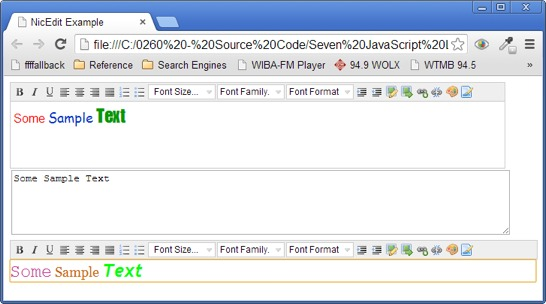
\includegraphics[width=13cm]{recursos/NicEdit/NicEdit.jpg}
\label{2}
\caption{NicEdit. Fonte:https://goo.gl/UZv5Sd; Acesso em 22/09/2017}
\end{figure}


\section{SummerNote}
Summernote é um editor de texto baseado no Bootstrap. Existem vários temas disponíveis para eles e eles são alimentados pelo Bootswatch. Há também uma versão convertida no tema Material chamado MaterialNote.

\subsection{Vantagens}
\begin{enumerate}
\item Fácil de instalar
\begin{itemize}
\item Basta baixar e anexar seu js, css com bootstrap.
\end{itemize}
\item Personalização
\begin{itemize}
\item Personalizar inicializando várias opções e módulos.
\end{itemize}
\item Exemplos
\begin{itemize}
\item Veja todas as características úteis do summernote em ação.
\end{itemize}
\item Código aberto
\begin{itemize}
\item Summernote é licenciado sob MIT e mantido pela comunidade em.
\end{itemize}
\item Integração
\begin{itemize}
\item Integre-o com qualquer back-end. 3 partes disponíveis no django, trilhos, angulares.
\end{itemize}
\end{enumerate}

\subsection{Como utilizar?}
\begin{enumerate}
\item Defina seu arquivo html com a notação de html5
\lstinputlisting{recursos/SummerNote/Step1.html}
\item Faça a inclusão das bibliotecas do pluguin no header do seu documento
\lstinputlisting{recursos/SummerNote/Step2.html}
\item Defina uma tag div com o id summernote para que o inicializador do plugin consiga ativar os recursos:
\lstinputlisting{recursos/SummerNote/Step3.html}
\item Inicialize o Summer note.
\lstinputlisting{recursos/SummerNote/Step4.html}
\end{enumerate}

\subsection{Resultado}

\begin{figure}[h]
\centering
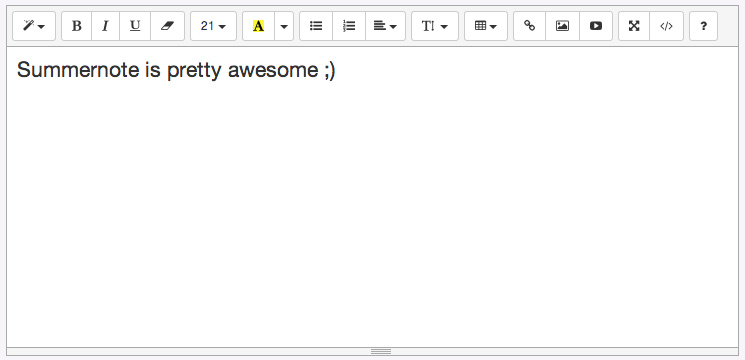
\includegraphics[width=13cm]{recursos/SummerNote/SummerNote.jpg}
\label{3}
\caption{SummerNote. Fonte:https://https://goo.gl/HjyaTd; Acesso em 22/09/2017}
\end{figure}



Gostou da ferramenta? Saiba mais em:


\url{https://summernote.org/getting-started/}


\url{https://summernote.org/}

\section{Bootstrap WYSIWYG editor}
O editor é baseado em browser execCommand, construído originalmente pela MindMup. 
O projeto possui licença MIT, é compatível com Chrome, Firefox e Safari, além de Windows, MAC e IOS e android.

\subsection{Vantagens}
\begin{enumerate}
\item Já utilizamos uma ferramenta bootstrap;
\item Open source;
\item Facilmente personalizável;
\item Arrastar e soltar arquivos para upload de imagem;
\item Formatação de texto fácil;
\item Não força qualquer uso de estilo; 
\item Suporta dispositivos móveis;
\item Não utiliza iFrames;
\item Leve. (5KB, menos de 200 linhas).

\end{enumerate}

\subsection{Como utilizar?}
\lstinputlisting{recursos/modelo/modelo.html}


\subsection{Resultado}
\begin{figure}[h]
\centering
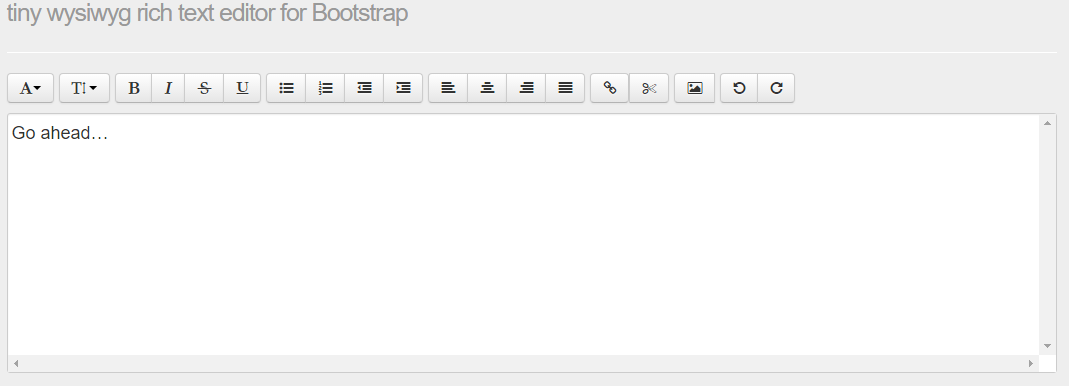
\includegraphics[width=15cm]{recursos/modelo/Bootstrap.png}
\label{4}
\caption{Bootstrap WYSIWYG. Fonte:http://mindmup.github.io/bootstrap-wysiwyg/; Acesso em 22/09/2017}
\end{figure}

Gostou da ferramenta? Saiba mais em: \url{http://mindmup.github.io/bootstrap-wysiwyg/}. E também um repositório no github: \url{https://github.com/mindmup/bootstrap-wysiwyg/} com mais informações sobre o editor.

\end{document}